\documentclass[a4paper,12pt]{article} % This defines the style of your paper

\usepackage[top = 2.5cm, bottom = 2.5cm, left = 2.5cm, right = 2.5cm]{geometry} 

\usepackage[T2A]{fontenc}
\usepackage[utf8]{inputenc}
\usepackage[russian]{babel}

\usepackage{multirow} 
\usepackage{booktabs} 

\usepackage{graphicx} 

\usepackage{setspace}
\setlength{\parindent}{0in}

\usepackage{float}

\usepackage{amsmath}

\usepackage{fancyhdr}

\usepackage{pgfplots}
\pgfplotsset{compat=1.9}

\pagestyle{fancy} 

\fancyhf{} 

\lhead{\footnotesize Расчетное задание №14}

\rhead{\footnotesize Николаев Юрий} 

\cfoot{\footnotesize \thepage} 

\begin{document}

\thispagestyle{empty} 

\begin{tabular}{p{15.5cm}} 
НИУ МЭИ \\ А-13а-19  \\ Вариант 13 \\ Николаев Юрий\\
\hline 
\\
\end{tabular} 

\vspace*{0.3cm}

\begin{center} 
	{\Large \bf Расчетное задание №14} 
	\vspace{2mm}
\end{center}  

\vspace{0.4cm}


\section{Задание}
Функция $y = y(x)$ задана таблицей своих значений. Применяя метод наименьших квадратов, приблизить ее функцией вида $\Phi(x) = a\varphi_0(x) + b\varphi_1(x)$. Определить величину среднеквадратичной погрешности. Построить на одном чертеже точечный график исходных данных и график функции $\Phi(x)$.

$$\varphi_0(x) = 1$$
$$\varphi_1(x) = x^2$$

\begin{center}
\begin{tabular}{| c | c | c | c | c | c | c |}
\hline
    x & 0,9 & 2,2 & 3,9 & 5,3 & 6 & 6,7 \\ \hline
    y & 3,562 & 4,368 & 6,442 & 9,018 & 10,6 & 12,378 \\
\hline
\end{tabular}
\end{center}

\section{Решение}

\begin{enumerate}

\item Функция $\Phi(x)$ имеет вид: $\Phi(x) = a + bx^2$.

\item Найдем нормальную систему МНК:

$$\sigma(\Phi_m, f) = \sqrt{\frac{1}{n + 1}\sum_{i = 0}^{n}(\Phi_m(x_i) - y_i)^2} = \sqrt{\frac{1}{n + 1}\sum_{i = 0}^{n}(a + bx_i^2 - y_i)^2}$$

\item Будем минимизировать функцию:

$$\bar \sigma(a, b) = \sum_{i = 0}^n(a + bx_i^2 - y_i)^2$$

Условие экстремума:

$$\frac{\partial \bar \sigma(a, b)}{\partial a} = 2\sum_{i = 0}^n(a + bx_i^2 - y_i) \cdot 1 = 0$$

$$\frac{\partial \bar \sigma(a, b)}{\partial b} = 2\sum_{i = 0}^n(a + bx_i^2 - y_i) \cdot x_i^2 = 0$$

Таким образом:
$$
\begin{cases}
    \sum_{i = 0}^n a + \sum_{i = 0}^n bx_i^2 = \sum_{i = 0}^n y_i \\
    \sum_{i = 0}^n ax_i^2 + \sum_{i = 0}^n bx_i^4 = \sum_{i = 0}^n y_i x_i^2 \\
\end{cases}
$$

$$
\begin{cases}
    6a + 129,84b = 46,368 \\
    129,84a + 4355,586b = 1312.5732 \\
\end{cases}
$$

Получаем коэффициенты системы: $a = 3,368982$; $b = 0,201433$.

Аппроксимирующая функция: $\Phi(x) = 3,368982 + 0,201433x^2$

\begin{center}
    $\Phi(0,9) = 3,532143$
    
    $\Phi(2,2) = 4,343918$
    
    $\Phi(3,9) = 6,432778$
    
    $\Phi(5,3) = 9,027235$
    
    $\Phi(6) = 10,62057$
    
    $\Phi(6,7) = 12,411309$
\end{center}

Считаем среднеквадратичное приближение: $\sigma = 0,0230012$



\begin{figure}[h]
\center{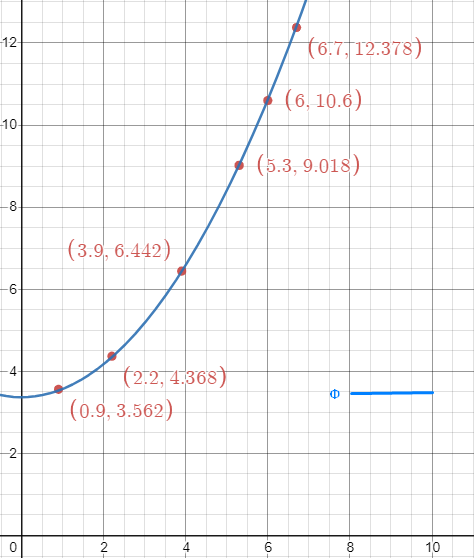
\includegraphics[scale=0.8]{graphic14.png}}
\caption{График}
\label{fig:image}
\end{figure}


\end{enumerate}

\end{document}